\claude{
\section{Further tests of practical decisions}\label{app:campaign}
We compare MG with scalar and task-specific baselines in six learning settings (Table~\ref{tab:campaign_scope}). Each study separates rule selection from evaluation. The settings address distinct decisions; their metrics do not measure a common dimension.

\begin{table}[htbp]
\centering\small
\caption{Scope of the additional studies. Values are from the final saved comparisons. Each row uses its own metric and evaluation population.}
\label{tab:campaign_scope}
\begin{tabularx}{\linewidth}{p{.20\linewidth}XX}
\toprule
Decision & MG result & Relevant comparison and scope \\
\midrule
SSL configuration selection & Mean Spearman $0.712$; top-choice regret $0.41$ pp & Embedding spread $0.730$; encoder RankMe $0.321$; five seeds, 29 configurations. \\
Transformer spike warning & $22/23$ events; AUROC $0.949$ & Roughness $23/23$, AUROC $0.960$ at the same false-positive rate; four test seeds. \\
Resetting after plasticity loss & Online accuracy $0.873/0.834$ in two task families & Dormant-neuron rule $0.880/0.843$; never resetting $0.845/0.776$; 12 streams per family. \\
Learning-rate reduction & Final accuracy $0.574$ & Fixed late reduction $0.590$; constant rate $0.543$; 24 evaluated runs. \\
Population-size proxy in games & Correct cycle category $0.523$ & Harmonic count $0.713$; state PCA about $0.99$; 216 new games. \\
Transfer of one detector & $26/87$ events; $10/58$ false positives & Detrended spread $85/87$; $9/58$ false positives across ten target settings. \\
\bottomrule
\end{tabularx}
\end{table}

\subsection{Self-supervised representation selection}
\paragraph{Task and architecture.}
We train an MNIST encoder with SimSiam, BYOL, VICReg or SimCLR objectives. The encoder is a 784--256--256 MLP with batch normalization and ReLU after each linear layer. Its representation is $h\in\mathbb R^{256}$. A 256--256--64 projector produces $z$; one configuration instead uses 16 output coordinates. SimSiam/BYOL usually use a predictor with hidden width 64. The 29 configurations vary step size, weight decay, augmentation strength, predictor, stop-gradient, projector normalization, loss coefficients, or contrastive temperature; the exact grid is bundled in \texttt{ssl/configs.py}.

Training uses 3,000 SGD steps, batch 128, momentum 0.9, and 100 warm-up steps followed by a constant learning rate. Two independently augmented images enter each update. The augmentation families combine affine shifts, rotations and scaling, erasure, pixel dropout, and Gaussian noise; their numerical ranges are in \texttt{ssl/ssl\_core.py}. These are small-model implementations of the published objectives \citep{chen2021simsiam,grill2020byol,bardes2022vicreg,chen2020simclr}, rather than reproductions of their original large-scale benchmarks.

\paragraph{Independent evaluation and information access.}
A logistic-regression probe fits standardized $h$ from 5,000 labeled training images with $C=0.1$ and at most 300 solver iterations. It is scored on 5,000 official test images. Fixed subsets use seed 1234. Their labels never enter SSL training. Probe accuracy supplies the target for choosing the monitor's log and direction on development seeds 0--1, then for scoring frozen selectors on test seeds 10--12. Seeds 20--21 add 58 further training runs after the initial comparison. Thus deployment of the selector is label-free, but its development is label-informed. The same probe images are reused across seeds, so this is a test of run variation on one task, not independent dataset generalization. The pilot seed 99 is excluded.

Each scalar selector chooses one of five recorded logs (loss, parameter norm, gradient norm, and representation/projector norms of one fixed image) and its sign using mean within-seed Spearman correlation on the development runs. No test outcome changes that choice. Primary MG uses $W=1{,}000$, $E=20$, $\tau=1$, $k=20$, and Theiler exclusion 19 on the final window. Its selected log is gradient norm and its sign is positive: higher MG predicts better representations in this task. This result concerns cross-run ranking, not an observed within-run dimension decrease. Undefined scores are ranked worst; no run is removed on the basis of downstream accuracy.

\paragraph{Representation proxies and scalar comparisons.}
RankMe \citep{garrido2023rankme} is computed separately on $h$ and $z$ from 2,048 images. The $\alpha$-ReQ comparison \citep{agrawal2022alphareq} uses a log--log slope fitted to the first 128 covariance eigenvalues of $h$, with both slope and distance-to-one variants. It does not reproduce the full search for a task-dependent preferred range in the original method. LiDAR \citep{thilak2024lidar} uses 256 images with eight augmentations each, evaluated on $z$, with within-image covariance ridge $10^{-4}$. Embedding spread is the mean coordinate standard deviation of unit-normalized $z$, multiplied by the square root of its dimension. Batch normalization can preserve a high encoder rank. Layer and augmentation choices also affect proxy quality, limiting this comparison to the specified implementations and grid.

All scalar methods receive the same candidate logs and development seeds. Competitors include roughness, recurrence error, spectral and permutation entropy, correlation dimension, TwoNN, delay covariance participation ratio, trend crossings, lag-one correlation, detrended spread, and level/change features. Table~\ref{tab:ssl_all} includes the complete frozen comparison.

\begin{table}[htbp]
\centering\small
\caption{SSL configuration ranking. Spearman correlations are computed across 29 configurations within each seed and then averaged. Regret is the gap between the chosen and best probe accuracy, averaged over five seeds and expressed in percentage points. The two confirmation seeds are shown separately.}
\label{tab:ssl_campaign}
\begin{tabular}{lrrrr}
\toprule
Score & Seeds 10--12 & Seeds 20--21 & All five & Regret (pp) \\
\midrule
MG (gradient norm) & 0.755 & 0.649 & 0.712 & 0.41 \\
Embedding spread & 0.729 & 0.732 & 0.730 & 1.46 \\
Spectral entropy & 0.653 & 0.507 & 0.595 & 1.00 \\
Roughness & 0.588 & 0.616 & 0.599 & 1.20 \\
Delay covariance PR & 0.652 & 0.587 & 0.626 & 1.08 \\
Correlation dimension & 0.540 & 0.674 & 0.594 & 0.75 \\
Recurrence error & 0.540 & 0.376 & 0.474 & 18.13 \\
RankMe ($h$) & 0.328 & 0.312 & 0.321 & 4.00 \\
RankMe ($z$) & 0.493 & 0.564 & 0.522 & 1.46 \\
$\alpha$-ReQ slope & 0.413 & 0.389 & 0.404 & 1.46 \\
LiDAR ($z$) & 0.120 & 0.130 & 0.124 & 85.03 \\
\bottomrule
\end{tabular}

\end{table}

\begin{figure}[htbp]
\centering
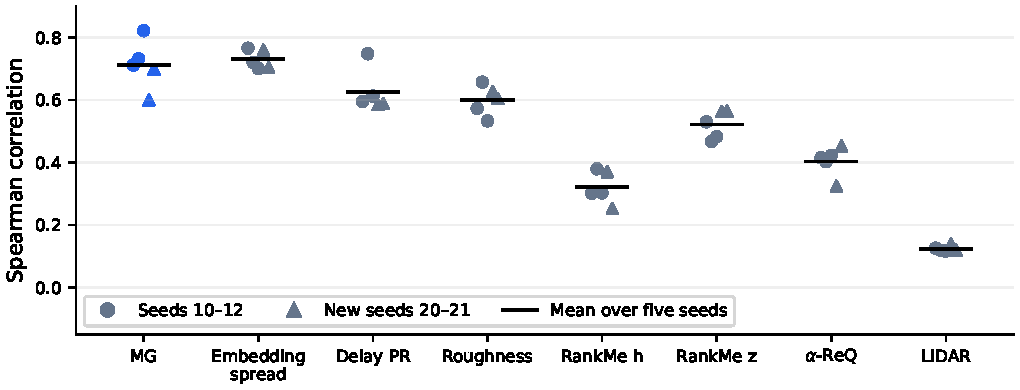
\includegraphics[width=.94\linewidth]{figures/ssl_campaign.pdf}
\caption{SSL ranking on individual seeds. Circles are the initial test seeds; triangles are the two later seeds. Horizontal bars show five-seed means. MG retains useful ranking on seeds 20--21, while embedding spread has the higher pooled mean.}
\label{fig:ssl_campaign}
\end{figure}

\paragraph{Results and uncertainty.}
MG has mean top-choice regret 0.408 percentage points versus 5.467 for random selection. Its ranking correlation falls from 0.755 on seeds 10--12 to 0.649 on seeds 20--21; embedding spread gives 0.729 and 0.732. Table~\ref{tab:ssl_campaign} reports the pooled means.

The archived pairwise intervals resample the 29 configurations with replacement, sharing each draw across all five seeds (1,000 replicates, RNG seed zero). They are pointwise intervals conditional on these seeds, with no correction for comparing many methods. They exclude zero against encoder RankMe, the slope version of $\alpha$-ReQ, LiDAR, and recurrence error; they include zero against projector RankMe, embedding spread, roughness, and spectral entropy. Table~\ref{tab:ssl_intervals} preserves these intervals without interpreting them as seed-level significance.

\begin{table}[htbp]
\centering\small
\caption{Archived 95\% pointwise configuration-bootstrap intervals for mean $\rho_{\rm MG}-\rho_{\rm comparison}$. Seed uncertainty and multiple comparisons are not accounted for by these intervals.}
\label{tab:ssl_intervals}
\begin{tabular}{lrr}
\toprule
Comparison & $\Delta\rho$ lower & $\Delta\rho$ upper \\
\midrule
Embedding spread & -0.192 & 0.190 \\
Spectral entropy & -0.050 & 0.330 \\
Roughness & -0.099 & 0.363 \\
Delay covariance PR & -0.073 & 0.304 \\
Correlation dimension & -0.050 & 0.326 \\
Recurrence error & 0.035 & 0.446 \\
RankMe ($h$) & 0.078 & 0.771 \\
RankMe ($z$) & -0.025 & 0.461 \\
$\alpha$-ReQ slope & 0.042 & 0.613 \\
LiDAR ($z$) & 0.180 & 1.053 \\
\bottomrule
\end{tabular}

\end{table}

\begin{table}[htbp]
\centering\small
\caption{All frozen SSL selectors over the five evaluated seeds. Score signs and logs were chosen only on development runs. The secondary MG setting uses $\tau=4,k=50$.}
\label{tab:ssl_all}
\begin{tabular}{lrrr}
\toprule
Statistic & Log & Mean $\rho$ & Regret (pp) \\
\midrule
MG & grad\_norm & 0.712 & 0.41 \\
out\_std & out\_std & 0.730 & 1.46 \\
spectral\_entropy & grad\_norm & 0.595 & 1.00 \\
linear\_pr & grad\_norm & 0.626 & 1.08 \\
crossings & loss & 0.586 & 1.02 \\
MG\_t4k50 & loss & 0.622 & 1.60 \\
roughness & loss & 0.599 & 1.20 \\
mean & grad\_norm & 0.548 & 3.15 \\
corr\_dim & loss & 0.594 & 0.75 \\
self\_repeat & grad\_norm & 0.474 & 18.13 \\
rel\_change & grad\_norm & 0.539 & 1.92 \\
lag1 & loss & 0.565 & 1.40 \\
rankme\_z & rankme\_z & 0.522 & 1.46 \\
rel\_std & grad\_norm & 0.482 & 1.17 \\
twonn & param\_norm & 0.459 & 85.03 \\
perm\_entropy & probe\_h\_norm & 0.431 & 85.03 \\
abs\_alpha1 & abs\_alpha1 & 0.404 & 1.46 \\
alpha\_h & alpha\_h & 0.404 & 1.46 \\
det\_std & probe\_h\_norm & 0.359 & 85.03 \\
rankme\_h & rankme\_h & 0.321 & 4.00 \\
recurrence\_rate & loss & 0.316 & 1.21 \\
lidar\_z & lidar\_z & 0.124 & 85.03 \\
\bottomrule
\end{tabular}

\end{table}

\paragraph{Failure detection, checkpoint selection, and cost.}
On seeds 10--12, a run is labeled unsuccessful when final probe accuracy falls below the mean random-initialization accuracy for the same seed plus 0.02. This definition measures weak downstream performance; it is not a proof of geometric collapse. Both the final and step-1,500 MG rules achieve AUROC 1.0, as do several other scalar rules. These detection rules select loss, rather than the gradient norm used for ranking. They were not confirmed on seeds 20--21. For checkpoint selection, spectral entropy has regret 0.00174, versus approximately 0.0069 for MG and 0.0172 for choosing the last checkpoint; this is another task with a separately fitted rule.

The saved CPU measurements average 30.83 ms for MG on a 1,000-sample window, versus 0.070 ms for roughness and 0.161 ms for spectral entropy. Gradient-norm logging needs no extra forward or backward pass, but its reduction is $O(P)$ and is not free. The archived RankMe time includes both $h$ and $z$ SVDs, and the original MG timing averages several logs under concurrent workers; these totals are not a fair single-score speed comparison. MG selection uses the saved log; embedding proxies require model access and image evaluations. Large-model scaling was not measured.

\subsection{Warning of slingshot loss spikes}
\paragraph{Model, event, and decision.}
We train a pre-layer-normalized transformer with two layers, width 64 and four heads on addition modulo 97, using Adam with zero weight decay for 8,000 steps. Inputs are two operands and a delimiter; the answer is predicted at the last position. Four configurations cross selected learning rates ($10^{-3}$ or $2\cdot10^{-3}$), second-moment coefficients (0.98 or 0.95), and training fractions (0.3 or 0.5). Batch size is 256 and warm-up lasts 100 steps. This produces slingshot events \citep{thilak2022slingshot}; a preliminary character-language-model pilot did not yield the desired events and is not the benchmark reported here.

An event begins when the next ten-step mean of $\log_{10}$ loss exceeds its preceding 200-step median by more than one and by more than six MAD-based standard deviations. Events have a 300-step exclusion interval. This use of future samples defines ground truth only. Monitors read completed 500-step windows every 50 steps, using loss or gradient/update/parameter norms; the first three are log-transformed. MG uses $E=20,\tau=1,k=20,T=19$. A successful warning occurs within 500 steps before onset. Windows ending at or within 500 steps after an onset are excluded from scoring; nearby false positives are merged within 500 steps. The false-positive rate is per 10,000 scored steps, not the entire training duration.

We choose the log, sign, threshold, and level/change rule using seeds 0--3, targeting at most two false positives per 10,000 steps, then evaluate seeds 10--13. The 16 test runs contain 23 scored events. The held-out false-positive rate need not meet the development constraint. Table~\ref{tab:spikes_campaign} includes all primary method comparisons.

\begin{table}[htbp]
\centering\small
\caption{Spike warnings on the held-out transformer runs. Hits are events warned within 500 steps; FP/10k counts merged false warnings per scored training steps. AUROC uses the frozen score and future-onset label at evaluation times.}
\label{tab:spikes_campaign}
\begin{tabular}{lrrr}
\toprule
Score & Hits & FP/10k & AUROC \\
\midrule
MG & 22/23 & 2.44 & 0.949 \\
MG\_t4k50 & 20/23 & 2.66 & 0.927 \\
self\_repeat & 23/23 & 2.76 & 0.960 \\
spectral\_entropy & 21/23 & 2.02 & 0.962 \\
roughness & 23/23 & 2.44 & 0.960 \\
perm\_entropy & 19/23 & 2.23 & 0.881 \\
recurrence\_rate & 20/23 & 2.44 & 0.726 \\
corr\_dim & 12/23 & 2.44 & 0.882 \\
twonn & 21/23 & 2.12 & 0.889 \\
linear\_pr & 23/23 & 2.66 & 0.959 \\
crossings & 17/23 & 2.44 & 0.841 \\
lag1 & 23/23 & 2.34 & 0.951 \\
det\_std & 23/23 & 2.76 & 0.931 \\
var & 22/23 & 2.44 & 0.923 \\
loss threshold & 23/23 & 2.34 & 0.946 \\
grad-norm threshold & 22/23 & 2.34 & 0.917 \\
update-norm level & 15/23 & 2.34 & 0.788 \\
param-norm level & 14/23 & 3.40 & 0.716 \\
INT attn-logit max & 4/23 & 1.70 & 0.645 \\
INT attn entropy & 15/23 & 1.59 & 0.911 \\
INT output logZ & 20/23 & 1.91 & 0.827 \\
\bottomrule
\end{tabular}

\end{table}

MG warns of 22/23 events with median lead 469.5 steps and precision 0.456. The long lead relative to the scoring horizon indicates an extended warning regime. Roughness warns of all events at the same false-positive rate for less computation. Attention scores are weaker for this slingshot mechanism; other instability mechanisms remain untested. Both the event definition and MG input use loss, so this is event forecasting rather than independent evidence of dimensional simplification. No intervention or training-quality improvement was tested.

\subsection{Reset rules, learning-rate schedules and transfer}
\paragraph{Plasticity and resets.}
Permuted-MNIST MLPs learn 40 successive tasks, 400 updates per task, with homogeneous or varying-noise input families. Rules select full-network resets at task boundaries. Development uses seeds 0--3, initial evaluation uses 10--14, and actual reset continuations use 20--21 crossed with six conditions, yielding 12 streams per family. MG improves online accuracy relative to never resetting, but dormant-neuron and weight-norm rules are better (Table~\ref{tab:campaign_scope}). The 12 streams are not 12 independent initialization seeds. 

\paragraph{Learning-rate decisions.}
A small CIFAR-10 CNN is trained under ten conditions varying batch size, initial step size, label noise, data volume, and budget. Development uses 12 runs and evaluation 24 runs. Each rule observes a constant-rate training path; saved checkpoints supply measured continuations with a tenfold rate reduction. MG reaches 0.574 final accuracy, improving on the constant-rate baseline, while the best fixed late reduction reaches 0.590. A second stop-after-reduction test gives only a 0.09 percentage-point advantage over a fixed schedule at matched average compute, with interval $[-0.34,0.45]$ percentage points. Stationarity of a log is therefore not sufficient to determine the best time to reduce the learning rate.

\paragraph{Games and detector transfer.}
The game study constructs weakly coupled matching-pennies cycles and predicts a cycle category as a proxy for choosing a population size. It does not run a downstream PSRO improvement experiment. MG classifies 52.3\% of 216 new games correctly; full-state PCA is nearly exact and a scalar harmonic count reaches 71.3\%. In a separate transfer study, a detector fitted on one MNIST MLP is applied across width, objective, precision, restart, and dataset changes. MG detects 26/87 events with 10/58 false positives, versus 85/87 and 9/58 for detrended spread. The original threshold does not transfer reliably across these settings.

}
